\section{Infinite Lattice Multiplication Factor}
\label{sec:infinite_lattice}

\subsection{Problem Statement}
\label{subsec:infinite_lattice_ps}

In an infinite lattice a reactor of infinite size is considered and therefore neutrons are not capable of leaking out of the system. An infinite lattice effectively removes the effects of geometry in neutron transport and characterizes the system entirely in terms of its material properties. Since the physics of an infinite lattice are greatly simplified an analytic analysis of the system is possible. Consequently, the infinite lattice problem is ideal for an initial analysis of any new computational method. 

To begin, the mathemtical formulation of an infinite lattice will be described. In matrix form the two-group neutron balance equations for an infinite lattice can be written as,
\begin{equation}
\label{eq:infinite_lattice_neutron_balance}
   \left(
    \begin{array}{cc}
     \Sigma_{a_1} + \Sigma_{1\rightarrow 2} & 0 \\
     -\Sigma_{12} & \Sigma_{a_2} 
    \end{array}
   \right)
   \left(
    \begin{array}{c}
     \phi_1 \\
     \phi_2
    \end{array}
   \right) 
   = \frac{1}{k_{\infty}}
   \left(
    \begin{array}{cc}
     \nu\Sigma_{f_1} & \nu\Sigma_{f_2} \\
     0 & 0 
    \end{array}
   \right)
   \left(
    \begin{array}{c}
     \phi_1 \\
     \phi_2
    \end{array}
   \right). 
\end{equation}  
Solving the system in \ref{eq:infinite_lattice_neutron_balance} for the infinite multiplication factor, the following analytic expression is obtained,
\begin{equation}
\label{eq:infinite_lattice_kinf}
   k = \frac{\Sigma_{a_2}\nu\Sigma_{f_1} + 
             \Sigma_{1\rightarrow 2}\nu\Sigma_{f_2}}{
              \Sigma_{a_2}\left(
               \Sigma_{a_1} + \Sigma_{1\rightarrow 2}\right)}.
\end{equation}
The infinite multiplication factor is a function of five material parameters. Since this thesis is concerned with the affect of uncertainties in input parameters on computer code outputs, variations in $k_{\infty}$ as a function its stochastic input variables are of interest. Assume all variation in $k_{\infty}$ can be attributed to its input cross sections, whose distributions follow a multivariate Gaussian. To obtain physical homogenized, two-group cross section values a real system must first be modeled in a transport code. The \ac{UAM} Benchmark is sought for this purpose \cite{UAM_Benchmark}. Specifically, the \ac{TMI} assembly is modeled using the two-step method described in \cite{TwoStep_Approach}. A total of 300 perturbed cross section sets were produced to obtain the few-group mean and covariance data used in the proceeding analysis. The cross section data is summarized in Table \ref{table:infintie_lattice_tmi_data}.      
\begin{table}[!htb]
\caption{\label{table:infintie_lattice_tmi_data} 
Two-group cross section data for an infinite TMI lattice.}
\centering
\begin{tabular}{||c||c|c|c|c|c|c|c||} 
\hline \hline
  &  &  & \multicolumn{5}{|c||}{\textbf{Correlation Coefficient Matrix}}  \\ \hline
  & \textbf{Mean} & \textbf{Standard Dev.} & $\Sigma_{a_1}$ & $\Sigma_{a_2}$ & 
  $\nu\Sigma_{f_1}$ & $\nu\Sigma_{f_2}$ & $\Sigma_{1\rightarrow 2}$ \\ \hline \hline
$\Sigma_{a_1}$ & 1.04E-02 & 9.06E-05 & 1 & 0.07 & -0.13 & 0.02 & 0.75 \\ \hline
$\Sigma_{a_2}$ & 1.10E-01 & 2.31E-04 & 0.07  &  1     & 0.06  & 0.31 & -0.07 \\ \hline
$\nu\Sigma_{f_1}$ & 9.00E-03 & 4.85E-05 & -0.13 &  0.06  & 1     & 0.33 & -0.10 \\ \hline
$\nu\Sigma_{f_2}$ & 1.91E-01 & 8.87E-04 & 0.02  &  0.31  & 0.33  & 1    & 0.01 \\ \hline
$\Sigma_{1\rightarrow 2}$ & 1.80E-02 & 2.18E-04 & 0.75  &  -0.07 & -0.10 & 0.01 & 1 \\ \hline \hline
\end{tabular}
\end{table}

Multiple methods will be applied to obtain basic statistical and sensitivity data on the infinite multiplication factor. Of course, Monte Carlo sampling using the input cross sections' covariance matrix and applying \ref{eq:sample_covariance} will provide the mean and variance of $k_{\infty}$. Another approach to get at the variance of $k_{\infty}$ is through the "Sandwich Equation"\cite{Jessee_Turinsky},
\begin{equation}
\label{eq:sandwich}
   \sigma^2(k_{\infty}) = S^TCS
\end{equation}      
where $C$ is the covariance matrix for the input data. In equation \ref{eq:sandwich} the array $S$ contains sensitivities of the output to the input parameters. For this problem the vector $S$ contains,
\begin{equation}
\label{eq:sensitivity_vector}
   S^T = \left(
    \begin{array}{ccccc}
     \frac{\partial k_{\infty}}{\partial\Sigma_{a_1}} &
     \frac{\partial k_{\infty}}{\partial\Sigma_{a_2}} &
     \frac{\partial k_{\infty}}{\partial\nu\Sigma_{f_1}} &
     \frac{\partial k_{\infty}}{\partial\nu\Sigma_{f_2}} &
     \frac{\partial k_{\infty}}{\partial\Sigma_{1\rightarrow 2}}
    \end{array}
         \right).
\end{equation} 
Since there exists an analytic expression for $k_{\infty}$ the sensitivity vector for this problem in \ref{eq:sensitivity_vector} is exact. As a side-check the sensitivity vector $S$ can also be constructed using central differencing. The sensitivity of $k_{\infty}$ to the $i^{\text{th}}$ cross section $\Sigma_i$ using central differencing is expressed as, 
\begin{equation}
\label{eq:central_diff_kinf}
   \frac{\partial k_{\infty}}{\partial \Sigma_i}\biggr\rvert_
   {\Sigma_{j\neq i} = \bar{\Sigma}_j}
    \approx \frac{k_{\infty}(\Sigma_i + \Delta\Sigma_i) - 
    k_{\infty}(\Sigma_i - \Delta\Sigma_i)}
    {2\Delta\Sigma_i}
\end{equation} 
where all cross sections $\Sigma_j$, $j\neq i$, are held at their mean values. Generally a one percent perturbation $\Delta\Sigma$ is sufficient to obtain accurate sensitivities although this rule of thumb is dependent on the smoothness of the objective function. With a variety of methods available to obtain sensitivities and statistical momements of $k_{\infty}$ it is possible to thoroughly assess the potential of a reduced order model.       
     
\subsection{Analysis}
\label{subsec:kinf_analysis}

Several elements of the methodologies described in Chapter \ref{chap:rom} will be tested in this section and compared to results obtained using analytic and Monte Carlo approaches. For all Smolyak sparse grids constructed the hypercube domain extends to six standard deviations in each random variable. Since $k_{\infty}$ is a function of only five random variables a sparse grid interpolant will be constructed without applying any function decomposition in order to demonstrate the accuracy and convergence of the method. The convergence criteria for the sparse grid interpolant is set such that the maximum hierarchical surplus at a given level is not to exceed $10^{-10}$. Both Clenshaw-Curtis and Gauss-Patterson abscissas are tested. 
\begin{figure}
\caption{ \label{fig:kinf_sg_convergence}
Convergence study of a five dimensional sparse grid interpolant for the  multiplcation factor of an infinite TMI lattice. The boxed numbers represent the current number of knots in the sparse grid.}
 \begin{center}
  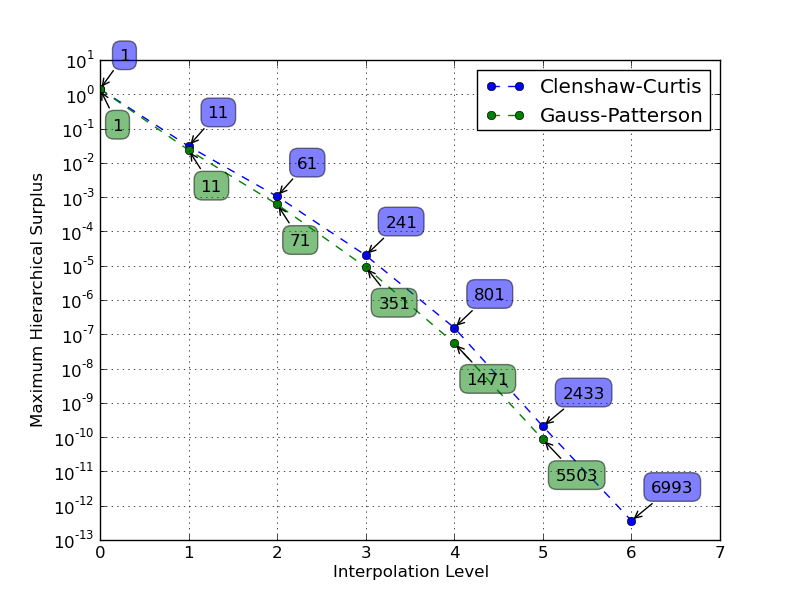
\includegraphics[scale=.75]{./Chapter3/kinf_sparse_grid_convergence.png}
 \end{center}
\end{figure}

From Fig. \ref{fig:kinf_sg_convergence} the Clenshaw-Curtis and Gauss-Patterson schemes perform similarly in terms of level to level convergence. However, observe that at each interpolation level the Gauss-Patterson scheme requires significantly more nodes in exchange for a small increase in convergence speed. Both schemes converge to the threshold around level five although the Gauss-Patterson scheme requires more than twice as many function evaluations to get there than Clenshaw-Curtis. Based on the graphical determination of order of convergence \cite{Boyd}, it is clear from \ref{fig:kinf_sg_convergence} that the Smolyak interpolant for $k_{\infty}$ converges geometrically.


% Full HDMR should exactly replicate . first order  

\begin{figure}
\caption{ \label{fig:kinf_numknots}
Cummultative number of knots required at each level of an anchored-\ac{ANOVA} decomposition of the multiplication factor of an infinite TMI lattice.}
 \begin{center}
  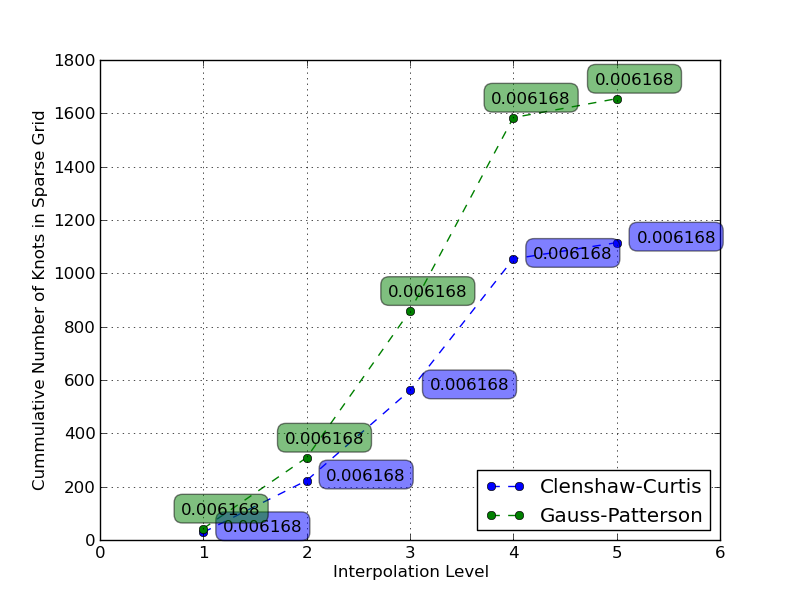
\includegraphics[scale=.75]{./Chapter3/kinf_sparse_grid_numknots.png}
 \end{center}
\end{figure}


\begin{table}[!htb] 
\caption{\label{table:kinf_mean_variance} 
Mean and variance data for the multiplication factor of an infinite TMI lattice. Wherever sampling was utilized the same random numbers were used.}
\centering
\small
\begin{tabular}{||c|c|c|c|c||} 
\hline \hline
\textbf{Method} & \textbf{Mean} & \textbf{95\% CI} & \textbf{Standard Dev.} & \textbf{95\% CI} \\ \hline
5D Sparse Grid CC      & 1.41562 & (1.41524, 1.41600) & 0.006168 & (0.005909, 0.006451) \\ \hline
5D Sparse Grid GP      & 1.41562 & (1.41524, 1.41600) & 0.006168 & (0.005909, 0.006451) \\ \hline
1D HDMR CC  & 1.41560 & (1.41522, 1.41598) & 0.006168 & (0.005909, 0.006451) \\ \hline
All HDMR CC & 1.41562 & (1.41524, 1.41600) & 0.006168 & (0.005909, 0.006451) \\ \hline
1D HDMR GP  & 1.41560 & (1.41522, 1.41598) & 0.006168 & (0.005909, 0.006451) \\ \hline
All HDMR GP & 1.41562 & (1.41524, 1.41600) & 0.006168 & (0.005909, 0.006451) \\ \hline
Monte Carlo            & 1.41562 & (1.41524, 1.41600) & 0.006168 & (0.005909, 0.006451) \\ \hline
Sandwich               &         &                    & 0.006540 &                      \\
\hline \hline
\end{tabular}
\end{table}

% Why don't results match with sandwich formula (analytic sensitivities used, more samples caused convergence)?    

\begin{table}[!htb] 
\caption{\label{table:kinf_sensitivities} 
Normalized sensitivity coefficients for the multiplication factor of an infinite TMI lattice.}
\centering
\begin{tabular}{||c|c|c|c|c|c||} 
\hline \hline
  & \multicolumn{5}{|c||}{\textbf{Normalized Sensitivity Coefficient of $k_{\infty}$}}  \\ \hline
\textbf{Method} & $\Sigma_{a_1}$ & $\Sigma_{a_2}$ & $\nu\Sigma_{f_1}$ & $\nu\Sigma_{f_2}$ & $\Sigma_{1\rightarrow 2}$ \\ \hline
5D Sparse Grid CC  & -.367551 & -.776087 & .224060 & .776010 & .143491 \\ \hline
5D Sparse Grid GP  & -.367551 & -.776087 & .224060 & .776010 & .143491 \\ \hline
1D HDMR CC         & -.367556 & -.776098 & .224063 & .776020 & .143493 \\ \hline
All HDMR CC        & -.367551 & -.776087 & .224060 & .776010 & .143491 \\ \hline
1D HDMR GP         & -.367556 & -.776098 & .224063 & .776020 & .143493 \\ \hline
All HDMR GP        & -.367551 & -.776087 & .224060 & .776010 & .143491 \\ \hline
Analytic           & -.367520 & -.775956 & .224044 & .775956 & .143476 \\ \hline
Central Difference & -.367551 & -.776089 & .224060 & .776011 & .143492 \\
\hline \hline
\end{tabular}
\end{table}